\mode*

% slide with examples of vertical text spacing
\begin{frame}<presentation>{Examples of adjusting vertical text spacing on a slides}
The quick brown fox jumps over the lazy dog. The vertical space between this and the next paragraph is set to 0.25~cm.
\vspacebeamer[0.25cm] % default is 0.5 cm vertical space

The quick brown fox jumps over the lazy dog. The vertical space between this and  the next paragraph is set to 0.5~cm.
\vspacebeamer % default is 0.5 cm vertical space

The quick brown fox jumps over the lazy dog. The vertical space between this and the next paragraph is set to 1.0~cm.
\vspacebeamer[1.0cm] % set 1.0 cm vertical space

The quick brown fox jumps over the lazy dog. The quick brown fox jumps over the lazy do. The quick brown fox jumps over the lazy dog.
\end{frame}

% slide with bullet lists
\begin{frame}<presentation>{Example of a nested bullet list with custom spacing}
\begin{itemize}\setlength\itemsep{5ex} % set spacing to 4 times height of letter x
    \item first thing to mention
    \item second thing to mention
    \item third thing to mention
    \begin{enumerate}\setlength\itemsep{1ex} % set spacing to 1 times height of letter x
        \item 
        \item 
        \item 
    \end{enumerate}
    \item last thing to mention
\end{itemize}
\end{frame}

% slide with a full-slide image
\begin{frame}<presentation>[plain]
  \begin{columns} % place figure in column to remove the left margin
    \begin{column}{\paperwidth} % column width equal to paper width
      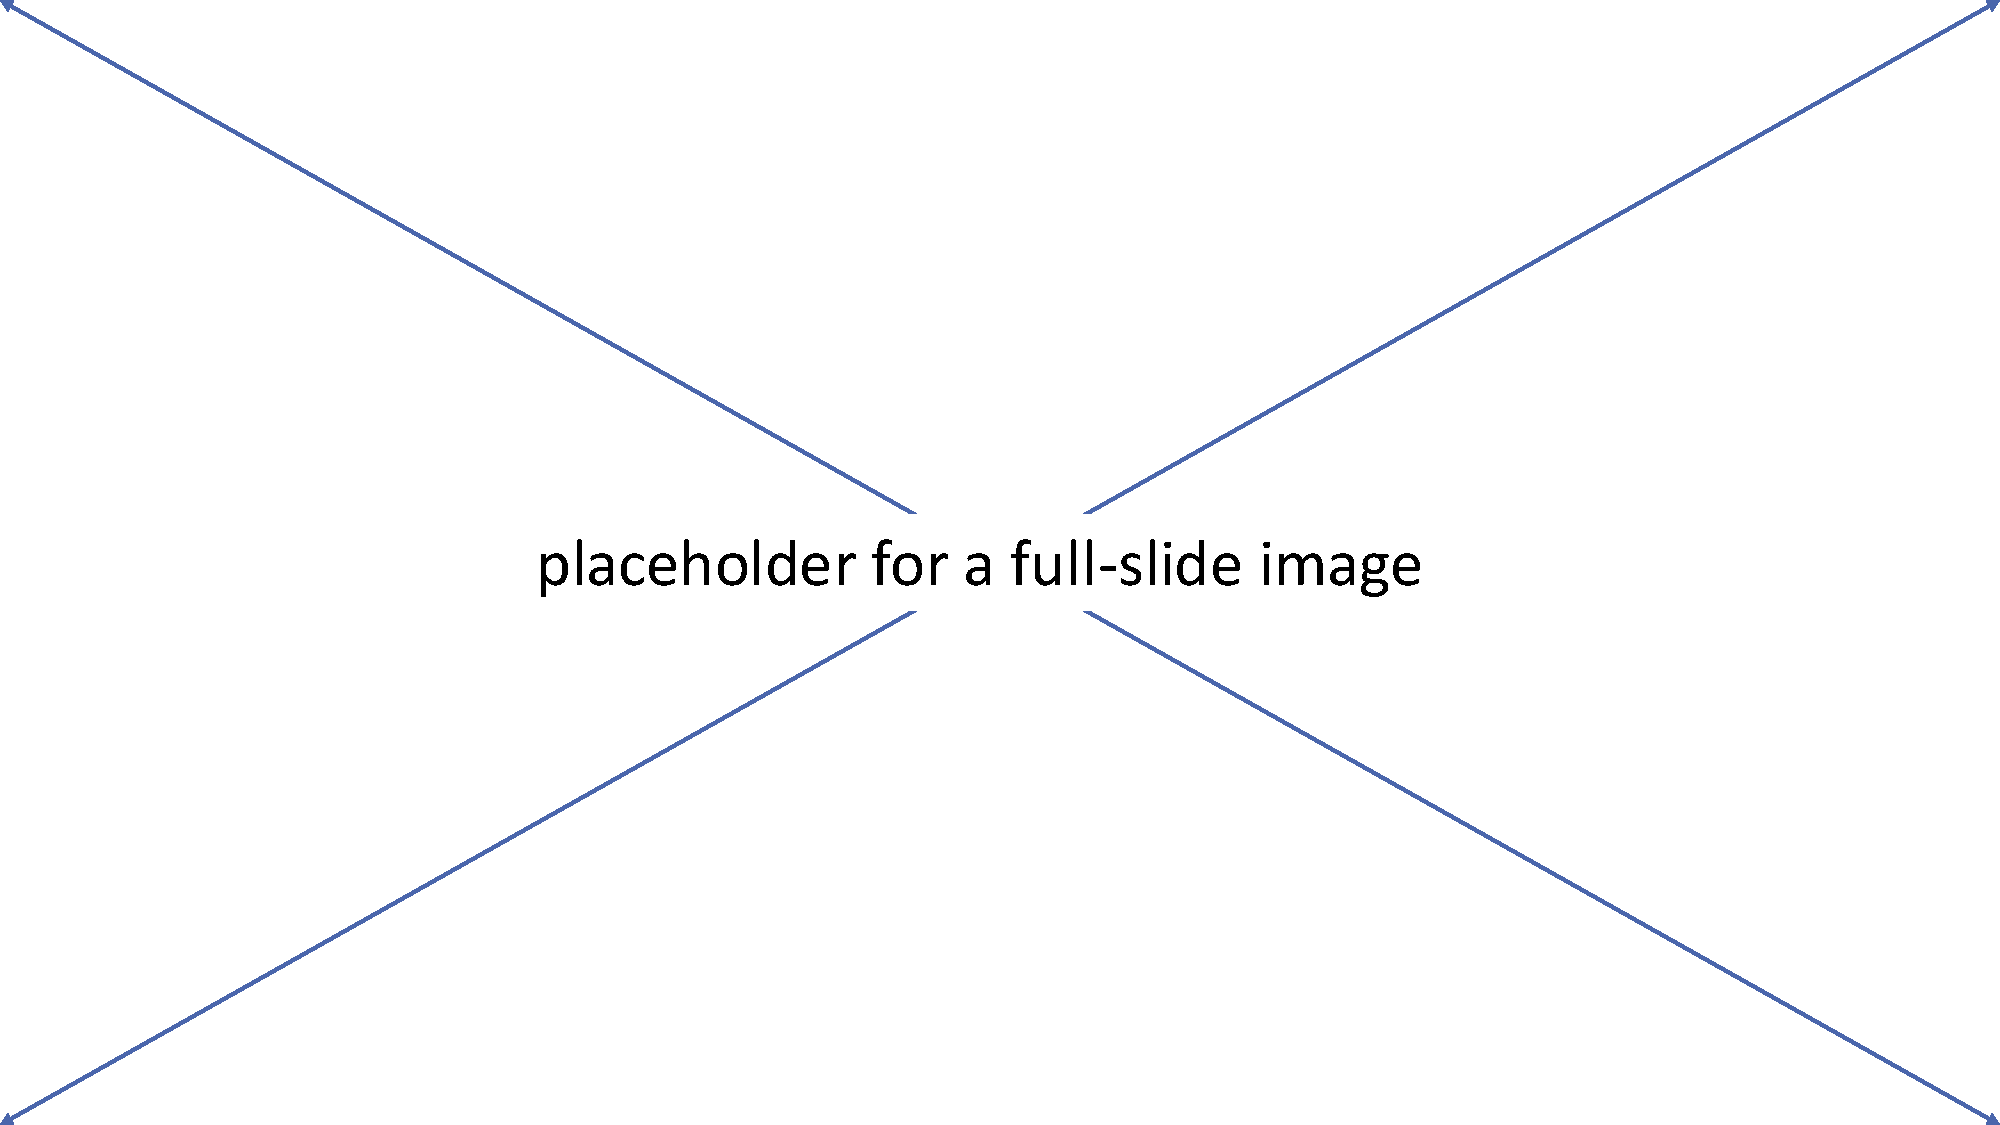
\includegraphics[height=\paperheight,width=\paperwidth]{figs/fullslideimage.pdf}
    \end{column}
  \end{columns}
\end{frame}

% slide with 2 columns
\begin{frame}<presentation>{Example of a slide with two columns}
 \begin{columns}    
    \begin{column}{0.5\textwidth} % resize if you wish
        \begin{figure}\centering
            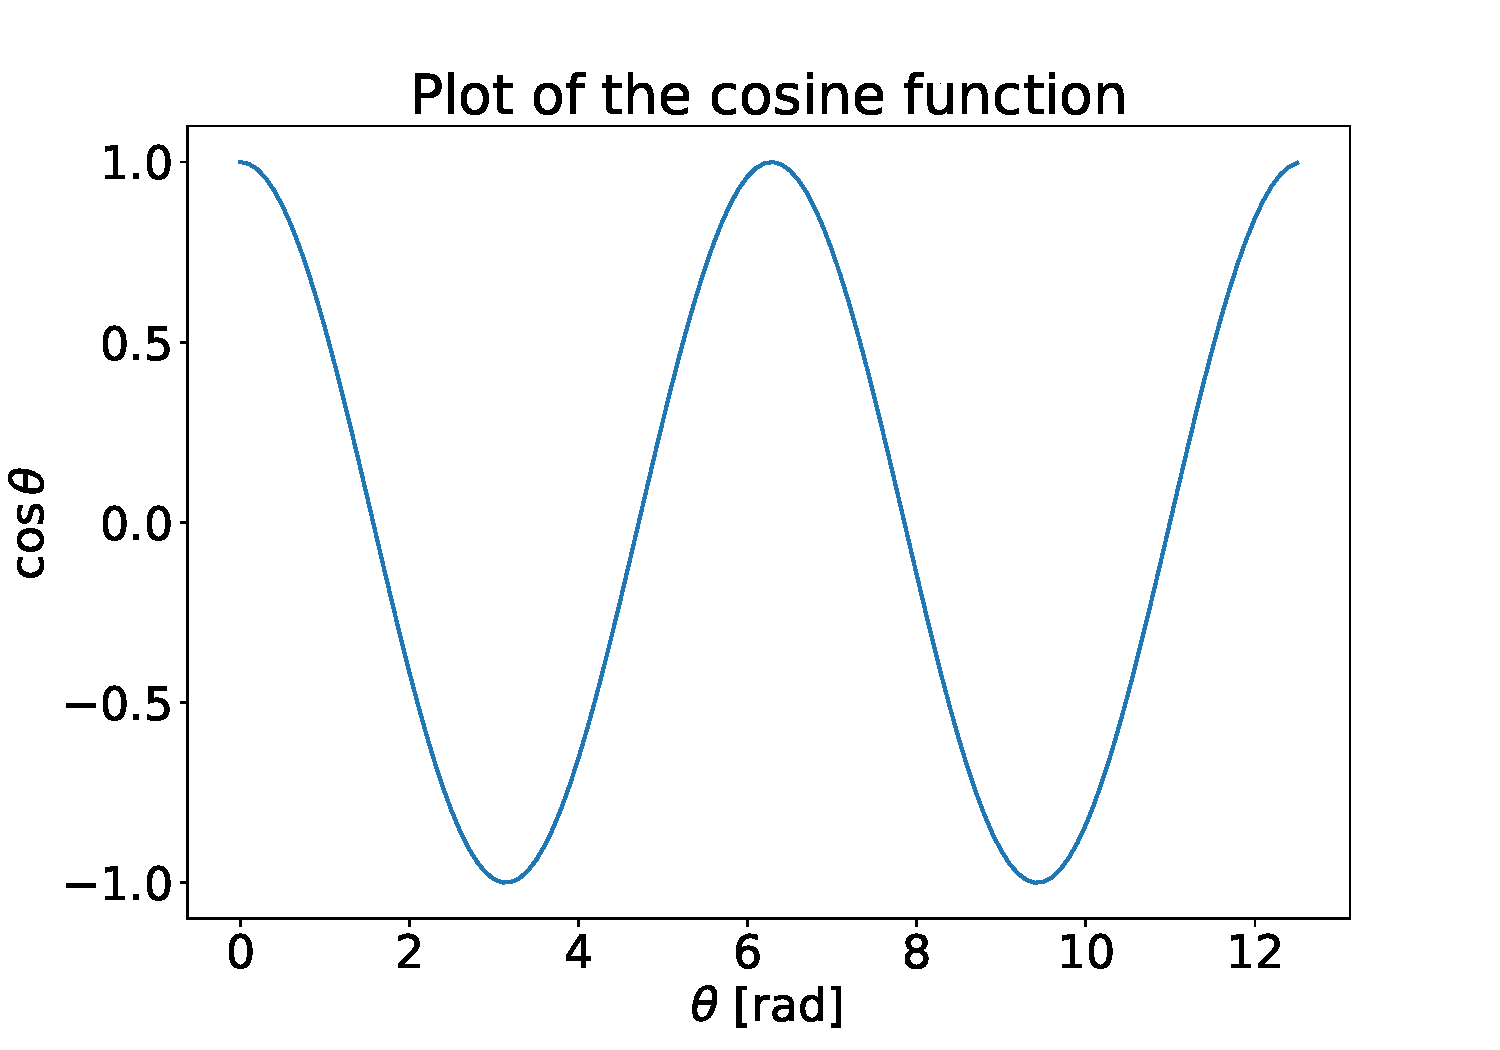
\includegraphics[width=\textwidth]{figs/cos.pdf}
            \caption{Some text}
        \end{figure}
    \end{column}
    \begin{column}{0.5\textwidth}  % resize if you wish
    \begin{align*}
        \intertext{Here you can provide extra info about the figure}
        \intertext{Equations can also easily be added}
        &\cos\theta\ \text{as function of}\ \theta
        \intertext{And some more info here}
        \intertext{And some more info here}
    \end{align*}   
    \end{column}
\end{columns}
\end{frame}

% slide with positioned blocks
% to avoid that these positioned blocks also appear in your report when compiling with memoir,
% you have to use \mode<presentation> around the frame environment
\mode<presentation>{
\begin{frame}{Example of a slide with three positioned blocks: one with a figure and two with text}
    \begin{textblock*}{7cm}(1cm,1cm)   % block width, x from left, y from top
    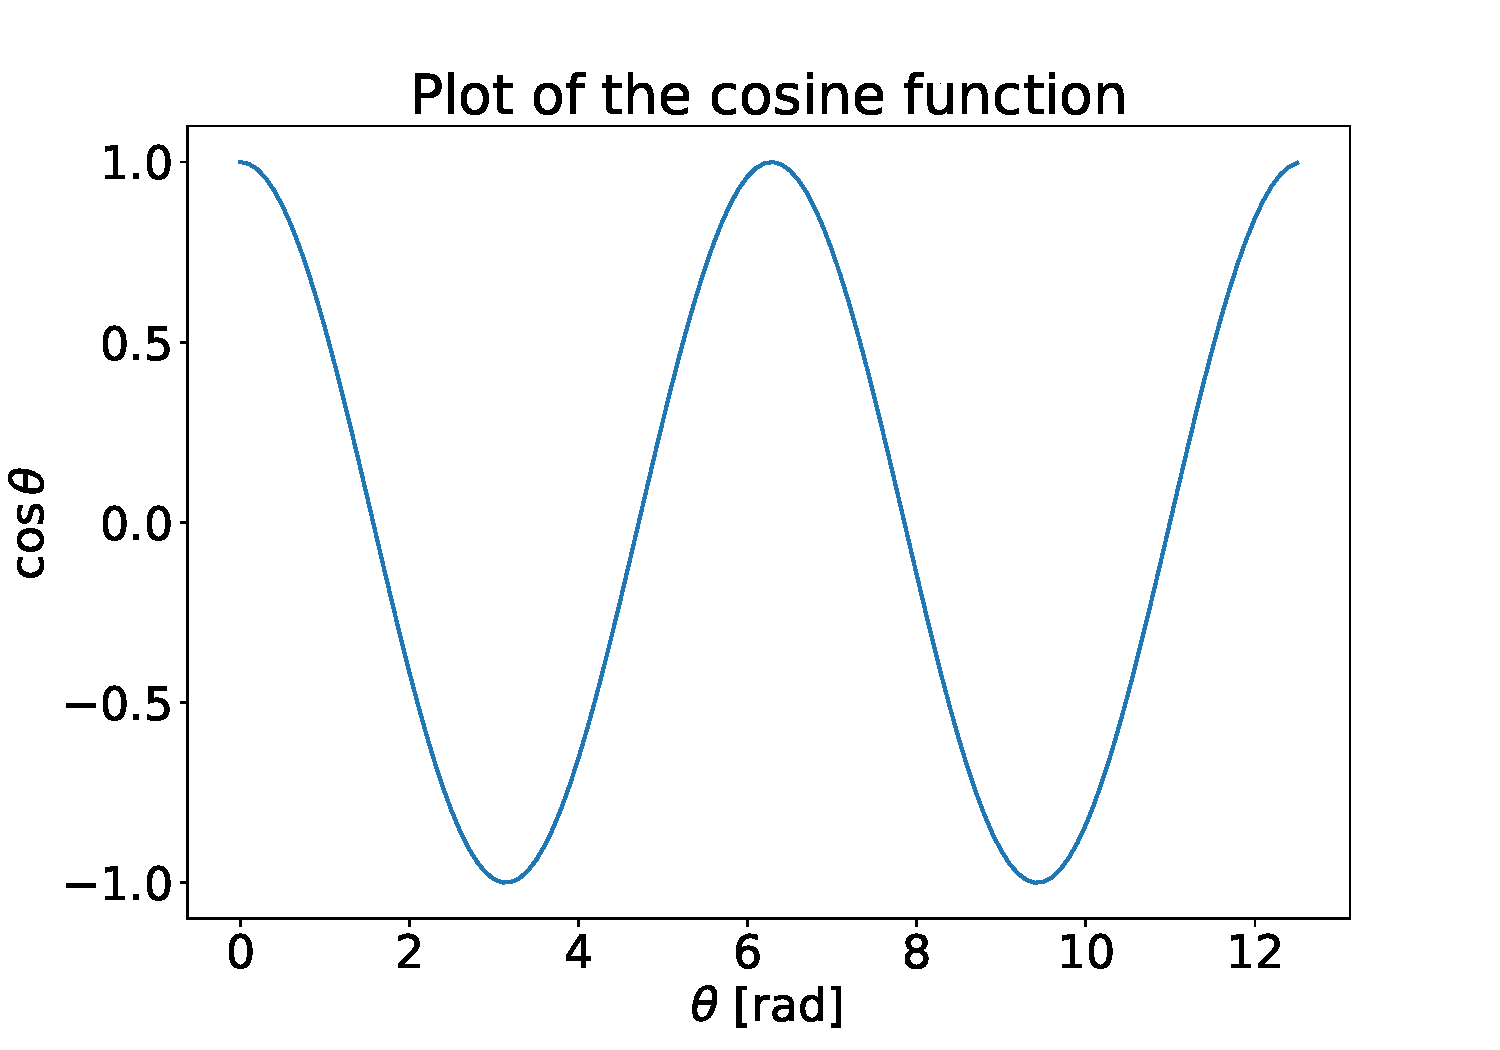
\includegraphics[width=\textwidth]{figs/cos.pdf}
    \end{textblock*}
    
    \begin{textblock*}{5cm}(8cm,2cm)   % block width, x from left, y from top
       A text block with given width positioned at location $x,y$ on the slide
    \end{textblock*}
    
    \begin{textblock*}{4cm}(3cm,6.5cm) % block width, x from left, y from top
       Another text block with given width positioned at another location $x,y$ on the slide
    \end{textblock*}
\end{frame}
}

\mode<all>


